%%%%%%%%%%%%%%%%%%%%%%%%%%%%%%%%%%%%%%%%%%%%%%%%%%%%%%%%%%%%%%%%%%%%%%
%%	Name: "Signal analysis template"
%%	File name: signalanalysis_template_main
%%	Version: 1.5
%%
%%	Compiler: XeLaTeX
%%
%%%%%%%%%%%%%%%%%%%%%%%%%%%%%%%%%%%%%%%%%%%%%%%%%%%%%%%%%%%%%%%%%%%%%%

\documentclass[conference,compsoc,onecolumn]{IEEEtran}

% *** LANGUAGE UTILITY PACKAGES ***
\usepackage[utf8]{inputenc} % Required for including letters with accents
\usepackage[spanish]{babel}
\usepackage{enumitem} % enumerados
\usepackage{graphicx}
\usepackage{subcaption}

% *** USED PACKAGES ***
% *** MISC UTILITY PACKAGES ***
\usepackage{comment}			% Agregar comentarios
\usepackage{lipsum}				% Inserts dummy text
\usepackage{blindtext}
\usepackage{listings}					% Coding
\usepackage{verbatim}				% Verbatim
\usepackage[final]{pdfpages}
\usepackage{booktabs,dcolumn}
\usepackage{pdflscape}
\usepackage{afterpage}
%\setlist[itemize]{noitemsep, nolistsep}
\usepackage[bookmarks=false]{hyperref}
\usepackage{tcolorbox}									% Coloured boxes, for LATEX examples and theorems, etc
\usepackage{color}
\usepackage{xcolor} % Required for specifying colors by name									% Color packages foreground and back­ground color man­age­men
% *** CITATION PACKAGES ***
\usepackage{cite}
% *** GRAPHICS RELATED PACKAGES ***
\usepackage{graphicx}
\usepackage{caption}
\usepackage{pgfplots}
\usepackage{tikz}
\usetikzlibrary{shapes,arrows}
\usetikzlibrary{decorations.pathmorphing} % noisy shapes
\usetikzlibrary{fit}					% fitting shapes to coordinates
\usetikzlibrary{backgrounds}	% drawing the background after the foreground
\pgfplotsset{compat=1.13}
% *** MATH PACKAGES ***
\usepackage{amsmath}
\usepackage{mathtools}
\usepackage{amssymb}
\usepackage{amsfonts}
\usepackage{expl3}
\usepackage{bm}

% *** SPECIALIZED LIST PACKAGES ***
\usepackage{algorithmic}
\usepackage{listings}					% Coding
\usepackage[framed,numbered,autolinebreaks,useliterate]{mcode}
% *** ALIGNMENT PACKAGES ***
\usepackage{array}
% *** SUBFIGURE PACKAGES ***
%\ifCLASSOPTIONcompsoc
%\usepackage[caption=false,font=normalsize,labelfont=sf,textfont=sf]{subfig}
%\else
%\usepackage[caption=false,font=footnotesize]{subfig}
%\fi
% *** FLOAT PACKAGES ***
\usepackage{fixltx2e}
\usepackage{stfloats}
%\fnbelowfloat
%\usepackage{dblfloatfix}
% *** PDF, URL AND HYPERLINK PACKAGES ***
\usepackage{url}
\usepackage{everypage}


\usepackage{multirow} % In order to be able to insert rows spanning multiple lines
\usepackage{verbatim}
\usepackage[all]{xy}
\usepackage{listings}
\usepackage{subfigure}
\usepackage{multibib}
\usepackage{setspace} 
\usepackage{algorithm}			    	  % To insert nice algorithms

% *** CARPETA DONDE SE GUARDARAN LAS IMAGENES ***
\graphicspath{{figures/}}

% *** NUEVOS COMANDOS Y CONFIGURACIONES VARIAS ***
\interdisplaylinepenalty=2500
\newcommand{\Lpagenumber}{\ifdim\textwidth=\linewidth\else\bgroup
	\dimendef\margin=0
	\ifodd\value{page}\margin=\oddsidemargin
	\else\margin=\evensidemargin
	\fi
	\raisebox{\dimexpr -\topmargin-\headheight-\headsep-0.5\linewidth}[0pt][0pt]{%
		\rlap{\hspace{\dimexpr \margin+\textheight+\footskip}%
			\llap{\rotatebox{90}{\thepage}}}}%
	\egroup\fi}

\AddEverypageHook{\Lpagenumber}%

\newcommand{\newtxt}[1]{\textcolor{black}{#1}}
\renewcommand\IEEEkeywordsname{Palabras cláve:}
\newcommand{\mx}[1]{\mathbf{\bm{#1}}} % Matrix command
\newcommand{\vc}[1]{\mathbf{\bm{#1}}} % Vector command

%% Separación de palabras
\hyphenation{op-tical net-works semi-conduc-tor HHMMSS}


\begin{document}

% *** TITLES AND NAMES ***
% title of the document
\title{Laboratorio 01: Introducción a \LaTeX}
% author names and affiliations
\author{\IEEEauthorblockN{Carlos Andres Arcila Quevedo\\Angel Fabian Nodarse \\Carla Sabrina Valdez}
\IEEEauthorblockA{Escuela de Ciencias Exactas e Ingeniería\\
	Universidad Sergio Arboleda - Bogotá, Colombia\\carlos.arcila@correo.usa.edu.co \\angel.nodarse@correo.usa.edu.co \\carla.valdez@correo.usa.edu.co }}


% *** MAKE TITLE ***
\maketitle
\IEEEoverridecommandlockouts
\IEEEpeerreviewmaketitle


\section{Introduccion }
Para  este  proyecto  se  planteo  el  uso  de  una  aplicacion  android  para  saber  el  posicionamiento  interior,  para  esto  se realizaran las respectivas investigaciones asi como el uso correcto de los documentos dados por el docente, como primer objetivo durante esta practica es entregar el debido documento con el contenido exigido por el docente durante esta misma. 
\section{Marco teórico}
\label{sec:marco}
\textbf{Sensores  en  smartphones }\\En el siglo XXI, uno de los equipos, en este caso, los mo ´viles son los mas utilizados, puesto que, facilitan la vida de los seres humanos con las diferentes aplicaciones y utilidades que brinda el equipo. Es  por  esto,  que  se  considera  relevante,  establecer  co ´mo  funciona  el  equipo  movil  y  sus  respectivos  sensores,  en este orden, como bien expone la pagina web computerhoy.com y su respectivo columnista Pascual (2018), el cual, manifiesta  que  los  sensores  son  aquellos  que  definen  al  dispositivo  movil,  y  es  una,  de  las  caracter´ısticas  que lo  diferencia  de  los  portatiles.Ademas,de  esto,  las  funciones  que  se  consideran  vitales  en  los  smartphones  estan asociadas a algu ´n sensor, dado que, condicionan el rendimiento de un movil, entre los sensores basicos estan: lector de huellas dactilares, acelero ´metro, magneto ´metro, giroscopio, GPS movil, sensor de proximidad o luz de ambiente; los cuales, son los mas comunes y utilizados en los smartphones. 
\\
\\
En este ambito, de acuerdo a la pagina web xataka.com (2019) , el acelerometro se considera como un componente mecanico, el cual, es similar a un chip; su tamaño reducido se debe a su nanotecnolog´ıa, y esta fabricado en silicio. La funcion del acelerometro, es para que el movil sepa en que  orientacion se encuentra, para que el dispositivo sepa cuando este, se ubica bien sea: horizontal, vertical o boca abajo. En lo que respecta, a los sensores capacitivos, este sensor es base para las pantallas tactiles actuales, estas, pantallas constan de un conductor transparente en la cual circula corriente de forma constante, y se encuentra aislado y/o cubierto por el cristal. Por otro lado, se encuentra el giroscopio , el cual, tiene como funcion complementar la informacion sobre la orientacion del movil, que ofrece el respectivo acelerometro. Es por esto, que se añade una cuarta dimension de movimiento, el cual tiene la funcion de medir la rotacion del movil; ademas de esto, cuando varıa su respectivo movimiento, estos son captados por un brazo de deteccion. 
\\
\\
Consiguiente  a  esto,  como  bien  expone,  la  pagina  web  xataka.com  (2019)  ,  los  sensores  de  GPS  que  tienen  los moviles,  se  encuentran  diseñados  con  el  objetivo  de  leer  de  manera  continua  las  sen ˜ales,  que  son,  transmitidas por  los  satelites  de  GPS.  De  esta  manera,  se  utiliza  de  manera  general  la  sen ˜al,  para  lograr  triangular  la  posicion del  dispositivo  movil.  Es  importante  recalcar,  que  dicha  señal  no  consume  datos,  pero  si  se  considera  mas  de ´bil en  espacios  tales  como  interiores  de  hogares,  es  por  esto,  que  es  mas  difıcil  medir  la  posicion  de  las  personas cuando  se  encuentran  dentro  del  hogar.  Por  lo  general,  los  GPS  que  tienen  los  moviles,  se  utilizan  respectivos angulos  de  interseccion,  de  al  menos  tres  satelites  respecto  del  movil  de  la  persona,  para  lograr  triangular,  donde esta , se encuentra. Ademas de esto, es vital recalcar que la funcion de GPS se puede desactivar de manera manual, en general, esta se desactiva cuando se es necesario ahorrar baterıa, dado que, si esta no se desactiva se seguira localizando de manera continua. 
\\
\\
Por  otro  lado,  segu n  la  pagina  web  xataka.com  (2019)  ,  el  lector  de  huellas  dactilar  tiene  una  serie  de  sensores capacitivos en una superficie, en donde, se pone el dedo; es aqu´ ı, donde el movil es capaz de reconocer las lıneas de las huellas dactilares de las personas, y almacenar una imagen digital de estas. De igual forma, este sensor es utilizado como un metodo biometrico, el cual colabora a la identificacion de los usuarios, consiguiente a esto, sirve 
para desbloquear el movil como bien se menciono  anteriormente, y la identificacion en aplicaciones. Ademas de lo anteriormente  expuesto,  el  movil  tambien  dispone  un  sensor  hall  o  magnetometro,  el  cual  se  constituye  como  un sensor electronico, el cual tiene como objetivo el medir y cuantificar las respectivas fuerzas magneticas, tambien, se le considera como una brujula electronica, puesto que, se puede configurar para detectar el polo norte magnetico de la tierra y de esta forma, definir en donde se encuentra el polo geografico; ası mismo, tiene funciones tales como: fundas que bloquean o que cambian el aspecto del movil.
\\
\\
Como  bien,  se  establece,  las  ideas  de  los  sensores  del  movil  y  su  utilidad,  de  acuerdo  a  las  ideas  expuestas  por la pagina web xataka.com (2019) , el sensor de proximidad tiene el objetivo de permitirle al movil, saber cuando este se encuentra en una cercanıa considerable del rostro de las personas, para apagar la pantalla. Puesto que, se encuentra compuesto por un LED infrarrojo, el cual emite un rayo invisible, este es, invisible al ojo humano, como tambien, un receptor de infrarrojo el cual tiene la capacidad de detectar la vuelta del rayo cuando ,este, rebota con una superficie. En este ambito, su funcionamiento se considera sencillo, y se basa en el tiempo que demora el rayo infrarrojo en volver, este sistema, es conocido como TOF (Time of Flight) o bien conocido como tiempo de vuelo. Es por esto, que, cuanto mas tarde la luz, significa que mas lejos estara el objeto. Las funciones que se encuentran asociadas a este sistemas son: apagar la pantalla cuando se acerca la cara para hablar, desbloqueo del movil al pasar la palma de la mano por encima, ademas de leer diversos gestos que se hacen con la mano sobre la pantalla. 
\\
\\
Consiguiente a esto, otro sensor que es valioso recalcar es el sensor de luz ambiental como bien expone la pagina web xataka.com (2019) , el cual tiene como objetivo detectar la cantidad de luz que se encuentra presente en el ambiente, es a partir de esto, que el movil es capaz de modular el brillo de la pantalla, cuando se tiene activada la opcion de brillo automatico, puesto que, se ajusta y modifica de forma diferente tanto en interiores como exteriores a partir de la luz base con la que se encuentre utilizando el dispositivo movil. Y por ultimo, el sensor infrarrojo, el cual esta, presente en algunos mo ´viles este tiene la funcion de controlar otros dispositivos que se encuentran en el hogar, a partir de un mando de distancia; esto, facilita el control del propio movil como de otros dispositivos, tales como: televisor o aire acondicionado, sin embargo, como bien se menciono, no todos los moviles lo traen.
\\
\\
\textbf{Sensores  en  smartphones }\\Un sistema de posicionamiento en interiores es una red de dispositivos utilizados para localizar  inala ´mbricamente  objetos  o  personas  dentro  de  un  edificio.   A  veces,  los  productos  que  se  ofrecen  bajo este termino no cumplen con la norma internacional ISO/IEC2 24730 sobre sistemas de localizacion en tiempo real ( RTLS ). En lugar de utilizar los satelites, un IPS se basa en anclajes proximos ( nodos con una posicion conocida ), que o bien localizan activamente etiquetas o bien proporcionan contexto ambiental a los dispositivos sensores. La naturaleza localizada de un IPS ha dado lugar a la fragmentacion de diseño, con sistemas haciendo uso de diversas tecnologıas : optica, de radio, o incluso acustica. 
\\
\\
\begin{itemize}

    \item La mayorıa de aplicaciones que necesitan de la ubicacion del usuario, utilizan una combinacion del sistema de geoposicionamiento global ( GPS ) y las redes moviles, esta combinacion funciona muy bien en exteriores, donde  la  cobertura  del  GPS  es  excelente  y  por  tanto  nos  permite  posicionarnos  rapidamente  y  de  manera muy exacta. Sin embargo, el GPS no funciona en interiores, y nos referimos a «  interiores »  no de un coche  ( porque en este caso sigue funcionando bien ), sino interiores de edificios, grandes centros comerciales, tiendas  etc.  Aunque  es  cierto  que  nos  posiciona  en  estos  lugares  (  por  las  redes  de  telefon´ıa  movil  ),  no lo  hace  con  exactitud  y  muchas  veces  el  terminal  movil  nos  indica  que  la  exactitud  es  de  1  kilometro de  distancia,  muchısimo  error  si  queremos  visitar  una  determinada  tienda  y  no  sabemos  do ´nde  esta.  Para solucionar el problema del geoposicionamiento en interiores, la Wi - Fi Alliance ha certificado el estandar Wi - Fi Location que nos va a permitir obtener datos de localizacion en interiores con una alta precision. El RSSI por ejemplo se puede utilizar, el RSSI indica la fuerza de la sen ˜al recibida por el dispositivo movil, cuanto mayor fuerza mas cerca esta ´  del punto de acceso Wi - Fi que le proporciona sen ˜al. La ubicacion en interiores  se  realiza  mediante  la  medicion  de  la  velocidad  de  las  ondas  de  radio  en  lugar  de  la  intensidad de la señal, ya que medir por el RSSI es bastante variable y limita la precision. Las señales Wi - Fi viajan a  traves  de  aire  a  la  velocidad  de  la  luz,  que  es  conocida,  por  tanto,  el  tiempo  entre  una  transmisio ´n  que sale de una antena de un AP hasta llegar al dispositivo movil se calcula facilmente ( Distancia = Velocidad de  la  luz  *  tiempo  ).  La  medicion  real  se  produce  cuando  el  AP  env´ıa  un  paquete  Wi  -  Fi  y  marca  su hora  de  salida,  cuando  el  cliente  recibe  el  paquete  tambien  marca  la  hora  de  llegada  y  calcula  el  tiempo que  ha  tardado  para  calcular  la  distancia.  Los  AP  que  esten  mas  libres,  o  que  tengan  mayor  ancho  de banda  para  los  clientes,  seran  los  que  mejor  informacion  de  posicionamiento  proporcionen.  Otro  aspecto muy importante es el problema del Multipath, es decir, si la señal Wi - Fi que recibimos es directa del AP o por el contrario la recibimos por otro camino ( rebotes de señal por ejemplo ). Por ultimo, la configuracion del AP es fundamental, y deberemos poner los datos de geoposicionamiento, incluyendo la altura y el piso si queremos que nuestros clientes sepan donde estan. 
     \\ \\Una  unidad  de  medicion  inercial  o  IMU,  es  un  dispositivo  electronico  que  mide  e  informa  acerca  de  la velocidad, orientacion y fuerzas gravitacionales de un aparato, usando una combinacion de acelerometros y giroscopos. La IMU es el componente principal de los sistemas de navegacion inercial usados en aviones, naves espaciales, buques y misiles guiados entre otros. En este uso, los datos recolectados por los sensores de  una  IMU  permiten  a  un  computador  seguir  la  posicion  del  aparato,  usando  un  metodo  conocido  como navegacion por estima. Por ejemplo, si una IMU instalada en un aeroplano informara que el aparato viajo hacia el oeste por una hora a una velocidad promedio de 804 kilometros por hora, el computador de guiado podrıa deducir que el avion deberıa estar a 804 kilometros al oeste de su posicion inicial. 
    \item El indicador de intensidad de señal recibida ( RSSI ) es una medida estimada de lo bien que un dispositivo puede o´ ır, detectar y recibir señales de cualquier punto de acceso o de un router espec´ıfico. Lo bueno de RSSI es  que  le  ayuda  a  determinar  y  saber  si  una  señal  es  suficiente  para  establecer  una  conexion  inalambrica. Este RSSI suele ser invisible para el usuario de un dispositivo receptor, pero como la intensidad de la señal varıa  enormemente  y  afecta  a  la  funcion  de  una  conexion  inalambrica,  los  dispositivos  a  veces  ponen  la medida a disposicion de los usuarios. 
    \item El fingerprinting tradicional tambien se basa en RSSI, pero simplemente se basa en el registro de la intensidad de  la  señal  desde  varios  puntos  de  acceso  dentro  del  alcance  y  el  almacenamiento  de  esta  informacion  en una base de datos junto con las coordenadas conocidas del dispositivo cliente en una fase fuera de lınea. Esta informacion puede ser determinista o probabilıstica. Durante la fase de seguimiento en lınea, el vector RSSI actual en una ubicacion desconocida se compara con los almacenados en la huella digital y la coincidencia mas cercana se devuelve como la ubicacion estimada del usuario. 
    \item Instrumento de aspecto parecido al de un reloj que, al llevarlo una persona encima, transforma en impulsos mecanicos o señales electricas las oscilaciones efectuadas por el cuerpo en la marcha y, ası, cuenta los pasos dados : sabiendo cual es la longitud media de sus pasos, una persona puede calcular con el podometro las distancias recorridas a pie. Su gran utilidad reside no solo en su medidor de pasos, si no en las diferentes funciones que presenta segun el modelo : calcula la distancia recorrida, las calorıas quemadas o el tiempo que hemos utilizado. Sinonimos : hodometro y odografo. Habitualmente se utiliza en el brazo, como un reloj de pulsera o en el cinturon, existen modelos de calidad superior que se usan en los tobillos o en los pies, estos  ultimos  llamados  acelerometros,  funcionan  a  traves  de  un  sensor  interno  que  detecta  el  movimiento de la mano y del cuerpo a la hora de caminar. 
\\
\\

\end{itemize}


\textbf{Beacon Bluetooth} Cuando se trata de posicionamiento de interiores combinado con tecnologıas 4.0, como el Internet of  Things  (IoT)  o  Internet  de  las  Cosas,  el  dıa  a  dıa  de  cada  persona  se  hace  mas  confortable  y  seguro.  Desde que el sistema de posicionamiento de interiores Estimote BLE (Bluetooth Low Energy) ha sido implementado para el  posicionamiento  de  un  smartphone,  provee  una  comunicacion  inalambrica  eficiente  en  potencia  comparado  al servicio de Bluetooth tradicional. Los faros BLE transmiten señales comunicando datos entre maestro y esclavo o mediante datos publicitarios a dispositivos. Generalmente, la baliza BLE es un pequeño transmisor desarrollado por Apple  y  otras  companıas  y  puede  ser  aplicado  en  varios  campos,  no  solo  para  encontrar  el  posicion  del  usuario interno, pero tambien para analizar la vida patrones o los patrones de consumo de los usuarios. En papel, diseñamos e implementamos el sistema de posicionamiento de interiores para estimar la posicion de un usuario con faros BLE y telefonos inteligentes. 
\\
\\
Mas especıficamente, los faros BLE son dispositivos transmisores utilizados para emitir una senal bluetooth de baja energ´ıa  (BLE)  a  dispositivos  moviles  que  se  encuentren  cerca  de  el  sin  necesidad  de  sincronizacion  previa.  Esta tecnolog´ıa permite a ejecutar determinadas acciones cuando telefonos inteligentes, ordenadores o tabletas entran en el radio de uno de ellos.
Los  faros  bluetooth  transmiten  un  identificador  unico  universal,  recogido  por  una  aplicacion  o  sistema  operativo compatible.  Esto  puede  utilizarse  para  determinar  la  ubicacio´n  fısica  del  dispositivo,  rastrear  objetos  o  activar acciones en funcion de la localizacion en determinados puntos de interes, como una parada de autobus, una tienda, una  localizacion  dentro  de  un  edificio,  etc.  A  diferencia  de  la  tecnologıa  GPS,  tiene  potencial  como  sistema  de posicionamiento en interiores y su consumo de baterıa es muy reducido.
En cuanto al hardware, la baliza BLE consiste en un microcontrolador con un chip de radio BLE y una baterıa, generalmente  de  boton.  Los  nuevos  chips  estan  optimizados  para  trabajar  con  BLE,  versiones  anteriores  fueron
 
diseñados con bluetooth clasico, lo que requerıa un mayor consumo de energıa.
\\
\\
El chip de radio BLE es generalmente fabricado por dos grandes empresas: Texas Instruments y Nordic Semiconduc- tor. Las bater´ıas de boto´n son las opciones ma´s populares para la mayor´ıa de estos dispositivos. Estas bater´ıas son densas  ce´lulas  de  iones  de  litio  y  proporcionan  desde  240  mAh  hasta  1000  mAh.  Dado  que  BLE  se  caracteriza por minimizar el uso de energ´ıa, la duracio´n de estas bater´ıas puede ser mayor a 1 an˜o. Algunos beacons tambie´n utilizan bater´ıas alcalinas AA.

\\
\\
Otros beacons funcionan externamente, se pueden instalar en una toma de corriente o un puerto USB, Estos dispositivos no necesitan un reemplazo de bater´ıas, con el inconveniente de la disponibilidad de una toma de corriente cercana. Los beacons transmiten una sen˜al con una potencia fija, conocida como Tx Power. A medida que la sen˜al viaja en el aire la  intensidad de la sen˜al va disminuyendo con la distancia.  Con un Tx Power superior la sen˜al puede viajar distancias ma´s largas, lo que significa mayor consumo y un Tx Power menor se traduce a menor rango de alcance pero menos consumo de bater´ıa.

\begin{itemize}
    \item iBeacon Es un protocolo creado por Apple, que se introdujo por primera vez en la Worldwide Developers Conference 2013. Apple fue la primera empresa que hizo conocida esta tecnolog´ıa a nivel mundial, pero la tecnolog´ıa (BLE) fue creada por Nokia. iBeacon utiliza BLE para transmitir un identificador u´nico universal (UUID) que es recogido por una aplicacio´n o sistema operativo compatible con el protocolo. El identificador ma´s  otros bytes  enviado  se pueden  usar para  identificar  la posicio´n  f´ısica  del dispositivo,  o  lanzar acciones basadas en la localizacio´n como notificacio´n push, etc.
    \\

iBeacon ofrece dos me´todos de API para detectar dispositivos ibeacons. Ranging, que solo funciona cuando la  aplicacio´n  esta´  activada  y  proporciona  estimaciones  de  proximidad;  Monitoring,  que  funciona  incluso  si la  aplicacio´n  no  esta´  corriendo,  y  proporciona  informacio´n  binaria  de  en  rango  y  fuera  de  rango.  iBeacons consta de cuatro piezas de informacio´n: UUID que identifica el beacon. Major es el nu´mero que identifica un subgrupo de beacons dentro de un grupo ma´s grande. Minor nu´mero de identificacio´n a un beacon espec´ıfico. La  aplicacio´n  de  escaneo  lee  el  UUID,  Major,  Minor  y  referencias  contra  una  base  de  datos  para  obtener informacio´n sobre el beacon, el propio beacon no lleva ninguna informacio´n descriptiva, requiere de una base de datos externa para ser u´til. El campo Tx Power se utiliza con la medida de la intensidad para determinar a que´  distancia se encuentra el beacon del dispositivo mo´vil (smartphone). Este campo tiene que ser calibrado beacon por beacon por el usuario para ser exacta.

\item EddystoneEs el proyecto de co´digo abierto de Google para beacons. Google, con esta tecnolog´ıa, pretende fomentar el internet de las cosas. Similar al protocolo de iBeacon pero open source. iBeacon esta´ soportado oficialmente por los dispositivos iOS solamente, Eddystone tiene soporte oficial para iOS y Android. Esta´  disen˜ado  para  soportar  mu´ltiples  tipos  de  paquetes  de  datos,  a  partir  de  Eddystone-UID  y  Eddystone-URL. Hay un tercer tipo de paquete de telemetr´ıa Eddystone-TLM. Este paquete se emite junto con Eddystone- UID  o  Eddystone-URL  y  contiene  el  estado  de  salud  del  beacon  como  por  ejemplo,  la  duracio´n  de  la bater´ıa.  Eddystone  se  basa  en  un  me´todo  u´nico  en  este  momento:  Eddystone  Discovery  que  es  similar  a iBeacon Ranging. Proporciona estimaciones de proximidad y solo funciona cuando esta´ activa. Google adema´s proporcionara´  las API  de  Nearby y  Proximity  para ayudar  a los  desarrolladores  en co´mo  transmitir datos  a equipos ubicados en el rango de los beacons seleccionados, a la vez que les permite monitorear los beacons. Cada trama de Eddystone debe contener los tipos de datos PDU: La lista completa de 16 bits de servicios UUID definido en Bluetooth Core Specification Supplement (CSS) v5. La lista de 16 bits debe contener el Eddystone Service UUID 0xFEAA. Esto es incluido para permitir el escaneo en segundo plano de dispositivos iOS. El tipo espec´ıfico de Eddystone frame se codifica en la parte alta de los cuatro primeros bits del primer byte de Service Data asociado con el Servicio UUID. Los valores permitidos son:
\\ \\
\begin{enumerate}
    \item UID 
    \item URL
    \item TML \\ \\
\end{enumerate}

\end{itemize}

\textbf{Trama de una Sen˜al wifi }Viene a ser el equivalente de paquete de datos o Paquete de red, en el Nivel de red del modelo OSI. La parte de datos es la que quiera transmitir en nivel de comunicacio´n superior, t´ıpicamente el Nivel de  red.  Para  delimitar  una  trama  se  pueden  emplear  cuatro  me´todos,  el  tracker  :  Habitualmente  se  emplean  STX ( Start of Transmission : ASCII 2 ) para empezar y ETX ( End of Transmission : ASCII 3 ) para terminar. Por
 
ejemplo  si  la  codificacio´n  f´ısica  es  bipolar  se  puede  usar  el  nivel  de  0  voltios,  o  en  Codificacio´n  Manchester  se puede tener la sen˜al a nivel alto o bajo durante todo el tiempo de bit ( evitando la transicio´n de niveles caracter´ıstica de este sistema ). FR Forum ( Asociacio´n de Fabricantes ) : Cisco, DEC, Stratacom y Nortel.
A fin de minimizar las interferencias entre tus dispositivos Wi - Fi y Bluetooth, se Para las estaciones base WiFi, restablecer  la  estacio´n  base  y  esta  intentara´  utilizar  los  canales  de  2,4  y  5  GHz  Conectarse  a  una  red  inala´mbrica de  5  GHz  (  si  es  posible  ).  Reducir  el  nu´mero  de  dispositivos  Bluetooth  inala´mbricos  activos  que  tengas  Si  el rendimiento en la red inala´mbrica no es o´ptimo por culpa de las interferencias para ello, alejar la base AP de los sitios excesivamente hu´medos, hornos microondas\\
\\

\begin{figure}[H]
    \centering
    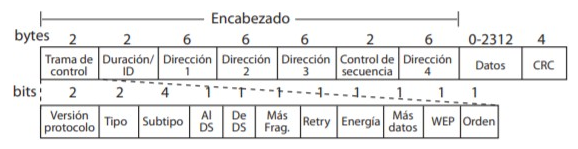
\includegraphics{bib/1.PNG}
    \label{fig:1}
\end{figure}


\textbf{Desarrollo movil} Son aquellas que se desarrollan de forma espec´ıfica para un sistema operativo determinado al que se conoce como Software Development Kit (SDK). Cada plataforma tiene un sistema operativo diferente. Los ma´s conocidos son iOS y Android. Tambie´n existen otros como Windows Phone. As´ı como manejan sistemas operativos diferentes,  tambie´n  utilizan  un  lenguaje  de  programacio´n  determinado.  Cuando  se  habla  del  lenguaje  de  sistema operativo, hacemos referencia a que:
\begin{enumerate}
    
    \item Las aplicaciones para Android se desarrollan en Java.
    \item Las aplicaciones para iOS se desarrollan en lenguaje Swift
    \item Las aplicaciones para Windows Phone antes se desarrollaban en .Net; ahora en C++ y Javascript.\\ \\

\end{enumerate}
La descarga o instalacio´n de las aplicaciones nativas se realiza desde las diferentes app stores de cada dispositivo. Es  importante  sen˜alar  que  las  app  nativas  no  necesitan  una  conexio´n  a  internet  para  su  funcionamiento.  Adema´s, las aplicaciones nativas esta´n capacitadas para adaptarse completamente a las funcionalidades del mo´vil y acceder a la mayor´ıa de caracter´ısticas hardware de este: ca´mara, agenda, GPS, etc.
\\
\\
El mayor inconveniente que podemos encontrar en el desarrollo de una aplicacio´n nativa es que tiene un coste ma´s elevado.  Como  indicamos  anteriormente,  hay  que  tener  en  cuenta  que  se  debe  realizar  una  aplicacio´n  para  cada sistema operativo. Eso hace que su precio se multiplique, dependiendo de los sistemas a los que queramos adaptar nuestra aplicacio´n.
\\
\\
\textbf{Web Apps o aplicacion web } El desarrollo de la aplicacio´n esta´ pensado para poder ejecutarla en cualquier dispositivo o  navegador.  Por  tanto,  la  aplicacio´n  estara´  programada  con  independencia  del  sistema  operativo.  A  diferencia  de la App Nativa, con una sola aplicacio´n web llegaremos a los diferentes dispositivos.
\\
\\
La Web Apps utiliza lenguajes muy conocidos entre los programadores como: HTML y CSS. Se ejecutan dentro del propio navegador web del dispositivo a trave´s de una URL. Una vez que deseas utilizarla, la propia aplicacio´n se adaptara´  al dispositivo que este´s usando. No necesitan instalacio´n, por lo que no siempre las encontraremos en los stores. Simplemente con crear un acceso directo, servir´ıa para usar dicha web app. Dos claros ejemplos son los accesos directos a Safari en iOS o Google Chrome en Android. Tiene una importante ventaja respecto a la App Nativa, su precio es ma´s econo´mico. Eso no significa garant´ıa de e´xito. Cuenta tambie´n con inconvenientes como la restriccio´n en el acceso a ciertas caracter´ısticas del dispositivo o la obligacio´n de tener conexio´n a internet para su utilizacio´n.
\\
\\
\textbf{Diagrama  de  casos  de  uso  del  sistema} En  Ingenier´ıa  del  Software,  es  una  te´cnica  para  la  captura  de  requisitos potenciales de un nuevo Sistema o una actualizacio´n de Software. Cada caso de uso proporciona uno o ma´s escenarios que  indican  co´mo  deber´ıa  interactuar  el  sistema  con  el  usuario  o  con  otro  sistema  para  conseguir  un  objetivo espec´ıfico.  Normalmente,  en  los  casos  de  usos  se  evita  el  empleo  de  jergas  te´cnicas,  prefiriendo  en  su  lugar  un lenguaje ma´s cercano al usuario final. Establece un acuerdo entre desarrolladores y clientes sobre las condiciones y posibilidades (requisitos) que debe cumplir el sistema. Artefacto narrativo que describe, bajo la forma de acciones y reacciones, el comportamiento del sistema desde el punto del usuario.
\\
\\
\textbf{Definicio´n  de  requisitos  del  software} Los  requisitos  se  han  convertido  en  un  punto  clave  en  el  desarrollo  de las  aplicaciones  informa´ticas.  Un  gran  nu´mero  de  proyectos  de  software  naufragan  debido  a  una  mala  definicio´n, especificacio´n  o  administracio´n  de  requisitos.  Factores  tales  como  requisitos  incompletos  o  mal  manejo  de  los cambios de los requisitos llevan a proyectos completos al fracaso total.
\\
\\
Debido a que los requisitos son las necesidades del producto que se debe desarrollar en cualquier proyecto de software, es importante no perder de vista que un requisito debe ser especificado por escrito como todo contrato o acuerdo entre dos partes; posible de probar o verificar para poder comprobar si se cumplio´  con e´l o no; consistente que no entre en contradiccio´n con otros requisitos y conciso, o sea, fa´cil de leer y entender. Adema´s, un requisito deber  estar  completo,  es  decir,  que  proporcione  la  informacio´n  suficiente  para  su  comprensio´n.  Y  por  u´ltimo  no debe ser ambiguo para no causar confusiones al lector.
\\
\\
En  la  definicio´n  de  requisitos,  se  averiguan  y  determinan  las  circunstancias  dif´ıciles  de  lo  que  se  debe  construir. Los requisitos funcionales se pueden clasificar en: normales, objetivos del sistema necesariamente presentes para la  satisfaccio´n  del  cliente;  esperados,  impl´ıcitos  al  sistema,  puede  que  el  cliente  no  los  declare  pero  de  no  estar no  cumple  con  su  estipulacio´n;  e  innovadores,  van  ma´s  alla´  de  la  expectativa  del  cliente,  los  puede  determinar  el desarrollador con el fin de no perjudicar lo pedido.
\\
\\
\textbf{Diagrama de actividades} Un diagrama de actividades muestra el flujo de actividades, siendo un actividad una ejecucio´n general entre los objetos que se esta´  ejecutando en un momento dado dentro de una ma´quina de estados, el resultado de un actividad es una accio´n que producen un cambio en el estado del sistema o la devolucio´n de un valor.  Las  acciones  incluyen  llamadas  a  otras  operaciones,  env´ıo  de  sen˜ales,  creacio´n  o  destruccio´n  de  objetos  o simples ca´lculos. Gra´ficamente un diagrama de actividades sera´  un conjunto de arcos y nodos. Desde un punto de vista conceptual, el diagrama de actividades muestra co´mo fluye el control de unas clases a otras con la finalidad de culminar con un flujo de control total que se corresponde con la consecucio´n de un proceso ma´s complejo. Por este  motivo,  en  un  diagrama  de  actividades  aparecera´n  acciones  y  actividades  correspondientes  a  distintas  clases. Colaborando todas ellas para conseguir un mismo fin. Ejemplo: Hacer un pedido.
\\
\\
\textbf{Contenido del diagrama de actividades} 
\begin{enumerate}
    \item Estados de actividad
    \item Estados de accio´n
    \item Transiciones
    \item Objetos
    \\
    \\
\end{enumerate}
\textbf{Estados de actividad y estados de accion} La representacio´n de ambos es un recta´ngulo con las puntas redondeadas, en  cuyo  interior  se  representa  bien  una  actividad  o  bien  una  accio´n.  La  forma  de  expresar  tanto  una  actividad como  una  accio´n,  no  queda  impuesta  por  UML,  se  podr´ıa  utilizar  lenguaje  natural,  una  especificacio´n  formal  de expresiones, un metalenguaje, etc. La idea central es la siguiente: “Un estado que represente una accio´n es ato´mico, lo  que  significa  que  su  ejecucio´n  se  puede  considerar  instanta´nea  y  no  puede  ser  interrumpida”,  Al  igual  que en el diagrama de estados, el de actividad cuenta con un punto inicial (representado por un c´ırculo) y uno final (representado como dos c´ırculos conce´ntricos).
\\
\\
En  cambio  un  estado  de  actividad,  s´ı  puede  descomponerse  en  ma´s  sub-  actividades  representadas  a  trave´s  de otros  diagramas  de  actividades.  Adema´s  estos  estados  s´ı  pueden  ser  interrumpidos  y  tardan  un  cierto  tiempo  en completarse. En los estados de actividad podemos encontrar otros elementos adicionales como son: acciones de entrada (entry) y de salida (exit) del estado en cuestio´n, as´ı como definicio´n de subma´quinas.
\\
\\
\textbf{Transiciones} Las transiciones reflejan el paso de un estado a otro, bien sea de actividad o de accio´n. Esta transicio´n se produce como resultado de la finalizacio´n del estado del que parte el arco dirigido que marca la transicio´n. Como todo flujo de control debe empezar y terminar en algu´n momento, podemos indicar esto utilizando dos disparadores de inicio y fin.
\\
\\
\textbf{Bifurcaciones} Un flujo de control no tiene porque´ ser siempre secuencial, puede presentar caminos alternativos. Para poder representar dichos caminos alternativos o bifurcacio´n se utilizara´  como s´ımbolo el rombo. Dicha bifurcacio´n tendra´  una  transicio´n  de  entrada  y  dos  o  ma´s  de  salida.  En  cada  transicio´n  de  salida  se  colocara´  una  expresio´n booleana que sera´  evaluada una vez al llegar a la bifurcacio´n, las guardas de la bifurcacio´n han de ser excluyentes
 \\
 \\
y  contemplar  todos  los  casos  ya  que  de  otro  modo  la  ejecucio´n  del  flujo  de  control  quedar´ıa  interrumpida.  Para poder  cubrir  todas  las  posibilidades  se  puede  utilizar  la  palabra  ELSE,  para  indicar  una  transicio´n  obligada  a  un determinado estado cuando el resto de guardas han fallado.
\\
\\
\textbf{Google App Engine} Google App Engine es un servicio de alojamiento web que presta Google de forma gratuita  hasta determinadas cuotas. Si no se cuenta con un dominio propio, Google proporciona uno con la siguiente estructura,  midominio.appspot.com.  Tambie´n  permite  implementar  un  dominio  propio  a  trave´s  de  Google  Apps. NET, Ruby y Go ) o usa tus propios frameworks y entornos de ejecucio´n de lenguajes. Gestiona recursos desde la l´ınea de comandos, depura el co´digo fuente en la fase de produccio´n y ejecuta backends de las API fa´cilmente con herramientas l´ıderes del sector, como el SDK de Google Cloud, Cloud Source Repositories, IntelliJ IDEA, Visual Studio y PowerShell.
\\
\\
\textbf{Bases de datos}Se define una base de datos como una serie de datos organizados y relacionados entre s´ı, los cuales son recolectados y explotados por los sistemas de informacio´n de una empresa o negocio en particular. 
\\
\\
1.	CARACTERISTICAS: Entre las principales caracter´ısticas de los sistemas de base de datos podemos mencionar:
\begin{itemize}
    \item Independencia lo´gica y f´ısica de los datos.
    \item Redundancia m´ınima.
    \item Acceso concurrente por parte de mu´ltiples usuarios.
    \item Integridad de los datos.
    \item Consultas complejas optimizadas.
    \item Seguridad de acceso y auditor´ıa.
    \item Respaldo y recuperacio´n.
    \item Acceso a trave´s de lenguajes de programacio´n esta´ndar.
    \\
    \\
\end{itemize}

Los  Sistemas  de  Gestio´n  de  Base  de  Datos  (  en  ingle´s  DataBase  Management  System  )  son  un  tipo  de  software  muy espec´ıfico, dedicado a servir de interfaz entre la base de datos, el usuario y las aplicaciones que la utilizan.
Control sobre la redundancia de datos : Sin embargo, en una base de datos no se puede eliminar la redundancia completa- mente, ya que en ocasiones es necesaria para modelar las relaciones entre los datos. Si un dato esta´ duplicado y el sistema conoce esta redundancia, el propio sistema puede encargarse de garantizar que todas las copias se mantienen consistentes.   La integridad de la base de datos se refiere a la validez y la consistencia de los datos almacenados. Estas restricciones se pueden aplicar tanto a los datos, como a sus relaciones, y es el SGBD quien se debe encargar de mantenerlas. Muchos   SGBD proporcionan lenguajes de consultas o generadores de informes que permiten al usuario hacer cualquier tipo de consulta sobre los datos, sin que sea necesario que un programador escriba una aplicacio´n que realice tal tarea. El SGBD proporciona muchas de las funciones esta´ndar que el programador necesita escribir en un sistema de ficheros. A nivel ba´sico, el SGBD proporciona todas las rutinas de manejo de ficheros t´ıpicas de los programas de aplicacio´n. El hecho de disponer de  estas  funciones  permite  al  programador  centrarse  mejor  en  la  funcio´n  espec´ıfica  requerida  por  los  usuarios,  sin  tener que preocuparse de los detalles de implementacio´n de bajo nivel. Sin embargo, los SGBD separan las descripciones de los datos de las aplicaciones. La mayor´ıa de los SGBD gestionan el acceso concurrente a la base de datos y garantizan que no ocurran problemas de este tipo. Sin embargo, los SGBD actuales funcionan de modo que se minimiza la cant.





\section{Diagrama de clases}
\label{sec:clases}

\begin{figure}[H]
    \centering
    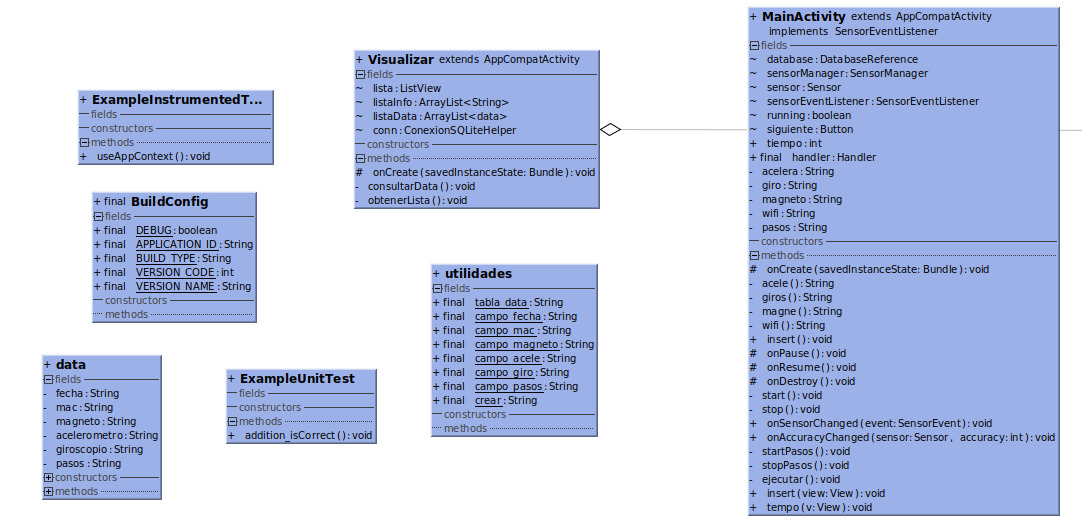
\includegraphics[scale=0.5]{bib/2.png}
    \label{fig:1}
\end{figure}

\section{Conclusiones}
\label{sec:conclusions}
A partir de las investigaciones exploradas, se puede puntualizar lo siguiente: los smartphones, utilizan sensores que facilitan la experiencia con el dispositivo mo´vil, dado que, estos controlan parte vital de este, ofreciendo herramientas para la orientacio´n del dispositivo, como de igual forma, brinda ubicaciones en tiempo real con la triangulacio´n de la posicio´n, ofrece un me´todo biome´trico para la identificacio´n de usuarios, dispone un sensor electro´nico,lo cual, facilita la deteccio´n de  las  respectivas  fuerza  magne´ticas.  Y,  por  u´ltimo,  es  importante  recalcar  que  maneja  un  sistema  como  TOF,  el  cual, facilita  la  activacio´n  de  un  LED  infrarrojo,  adema´s  de  esto,  maneja  el  sensor  asociado  al  medio  ambiente  para  modular la  luz  correspondiente  para  cada  espacio.  Por  otro  lado,  la  localizacio´n  en  interiores  se  constituye  como  un  sistema  para la  localizacio´n  de  personas  o  objetos,  aunque  este  no  funciona  a  gran  escala  y  es  poco  puntual  en  su  exactitud.  Y,  en esto, es importante resaltar que el LED infrarrojo no se encuentra disponible en todos los dispositivos mo´viles, dado que, adema´s de la funcio´n anteriormente mencionada, tambie´n tiene una comunicacio´n con la sincronicidad de otros dispositivos.
\\
\\
Consiguiente a esto, el BLE se constituye como un transmisor pequen˜o, para encontrar la posicio´n del usuario interno, pero  tambie´n  analiza  los  patrones  de  vida  o  los  patrones  de  consumo  de  los  usuarios,  este,  ofrece  beneficios  ma´s  que  el
 \\
 \\
GPS, dado que, tiene un potencial como sistema de posicionamiento en interiores y su consumo de bater´ıa es bajo, por otro lado, se encuentran, otros beacons los cuales son u´tiles, puesto que, no necesitan reemplazo de bater´ıas, transmiten una sen˜al con potencia fija conocida como Tx Power, este, puede viajar distancias ma´s largas. Es as´ı, que la trama de una sen˜al wifi esta´  constituida por paquetes de datos o paquetes de red, por lo cual, el desarrollo de mo´vil responde de forma espec´ıfica a un sistema operativa determinado conocido como (SDK), en este, los ma´s conocidos son: iOS, Android   Windows Phone, a estos, responden un lenguaje de programacio´n determinado.
\\
\\
De acuerdo a lo anterior, es importante resaltar que las aplicaciones nativas tienen ciertas limitaciones, una de ellas es su  costo  elevado,  puesto  que,  cada  aplicacio´n  necesita  un  sistema  operativo  espec´ıfico,  al  contrario,  de  las  Web  Apps  o aplicacio´n web , la cual , tiene como ventaja, que se puede ejecutar en cualquier dispositivo o navegador, es decir, con una sola aplicacio´n web se puede llegar a diferentes dispositivos, es en este escenario, que se hace vital un diagrama de casos de uso del sistema, dado que, se considera como una te´cnica para la captura de requisitos que son potenciales de un nuevo sistema  o  una  actualizacio´n  de  software,  es  decir,  proporciona  escenarios  sobre  co´mo  debe  interactuar  el  sistema  con  el usuario o con otro sistema para conseguir un objetivo espec´ıfico. Por otro lado, es vital considerar los requisitos, dado que, se postulan  como claves para  el desarrollo de  las aplicaciones informa´ticas, as´ı mismo,  en lo que  respecta a un  diagrama de  actividades,  esboza  de  manera  clara,  el  flujo  de  las  actividades  siendo  esta,  una  ejecucio´n  general  entre  los  objetos  de un momento dado dentro de una ma´quina de estado, el resultado de esto, efectu´a una accio´n que produce un impacto en el estado del sistema. En el dinamismo de un estado a otro, se desarrollan las transiciones, las cuales reflejan dichos cambios, as´ı mismo, se pueden presentar bifurcaciones, las cuales, se establecen como los caminos y/o escenarios alternativos de un flujo de control.
\\
\\
Todo lo anterior, se termina aglomerando en una base de datos, puesto que, esta´ se establece como una serie de datos organizados que se encuentran ´ıntimamente relacionados, los cuales, han sido recolectados por una empresa o negocio en espec´ıfico, el cual cuenta, con una lo´gica independiente, acceso de los usuarios, seguridad de acceso, consultas complejas y acceso a partir de lenguajes de programacio´n esta´ndar.
\\
Al momento de programar la aplicación como tal y de revisar todos los sensors necesarios para la generación del proyecto, se pudo evidenciar que ninguna APK de Android permite conocer el ruido de una señal Wi-FI por lo que optamos por mostrar en la data el RSSI que es la intensidad de la señal medida en decibels.
\\
\\
El uso de la nube como herramienta para de desarrollo abre un esapcio más amplio para el manejo de los datos y la adquisicion de información necesaria para el funcionamiento del sistema

\section{Anexos}

\begin{figure}[H]
    \centering
    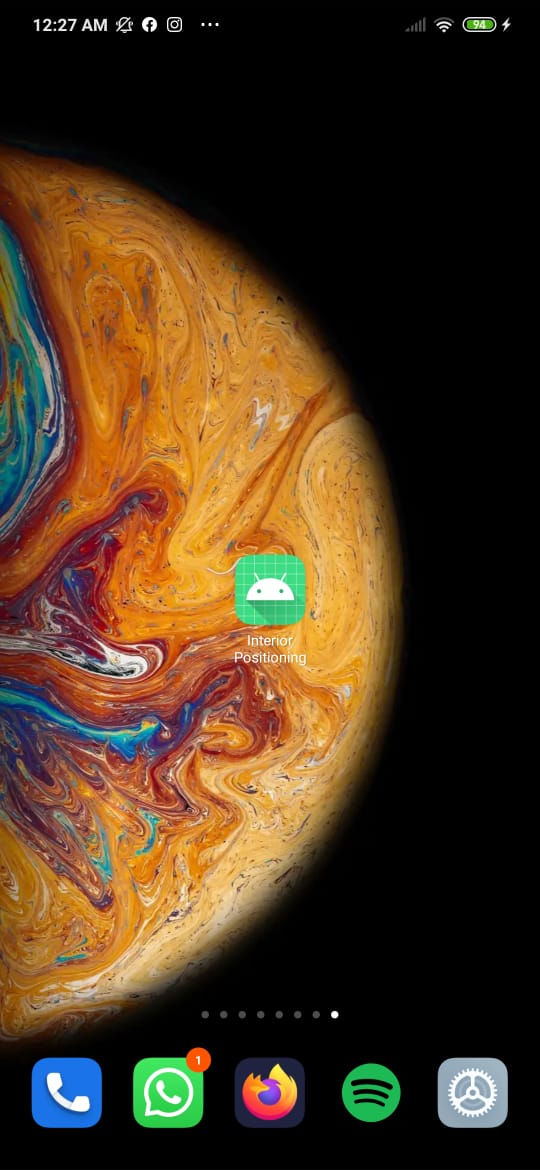
\includegraphics[scale=0.5]{bib/3.PNG}
    \label{fig:1}
\end{figure}

\begin{figure}[H]
    \centering
    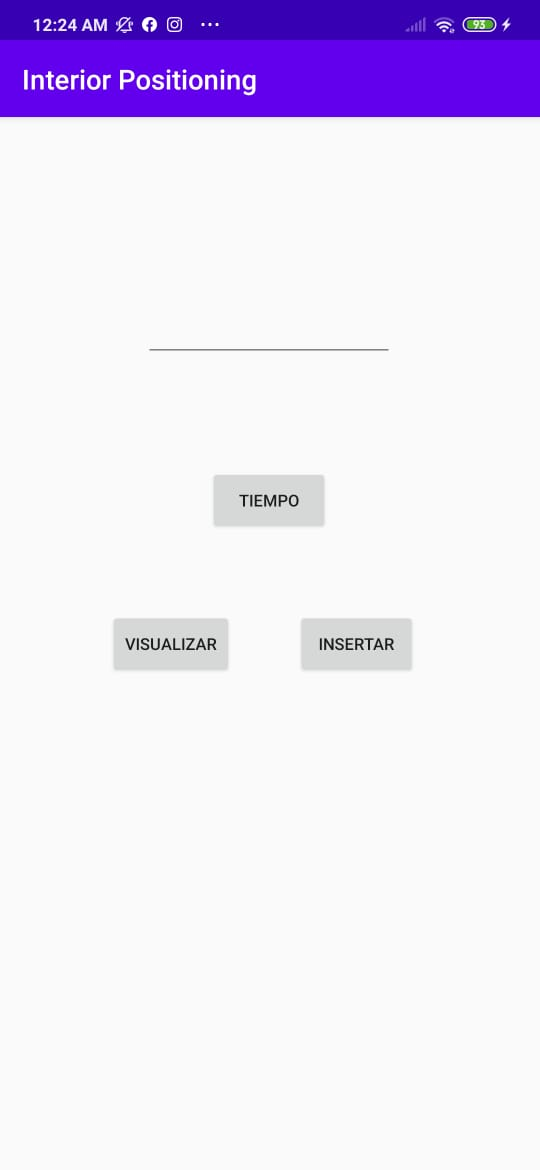
\includegraphics[scale=0.5]{bib/4.PNG}
    \label{fig:1}
\end{figure}
\begin{figure}[H]
    \centering
    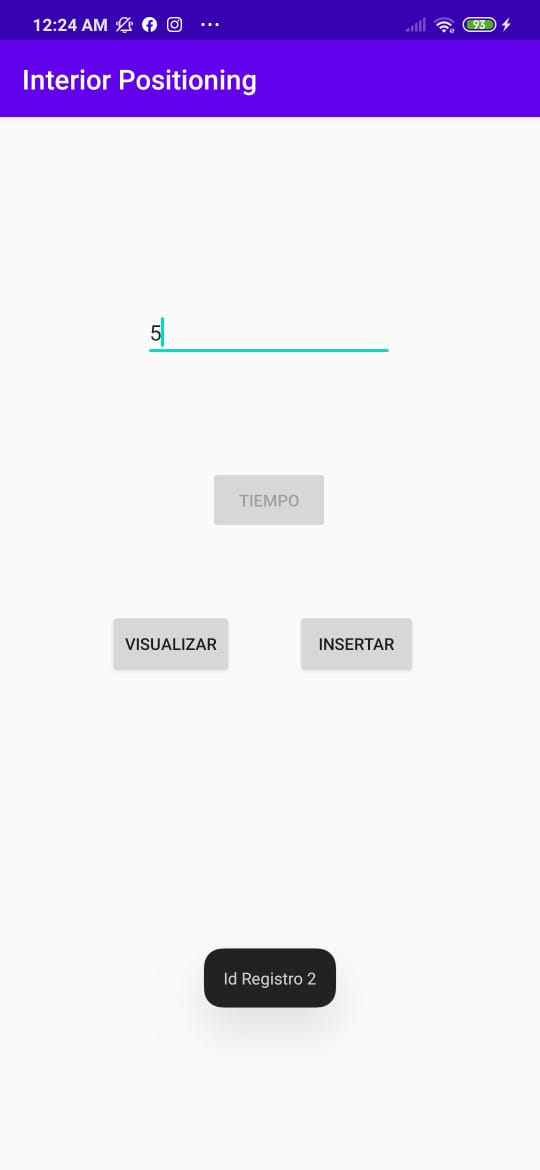
\includegraphics[scale=0.5]{bib/5.PNG}
    \label{fig:1}
\end{figure}

\begin{figure}[H]
    \centering
    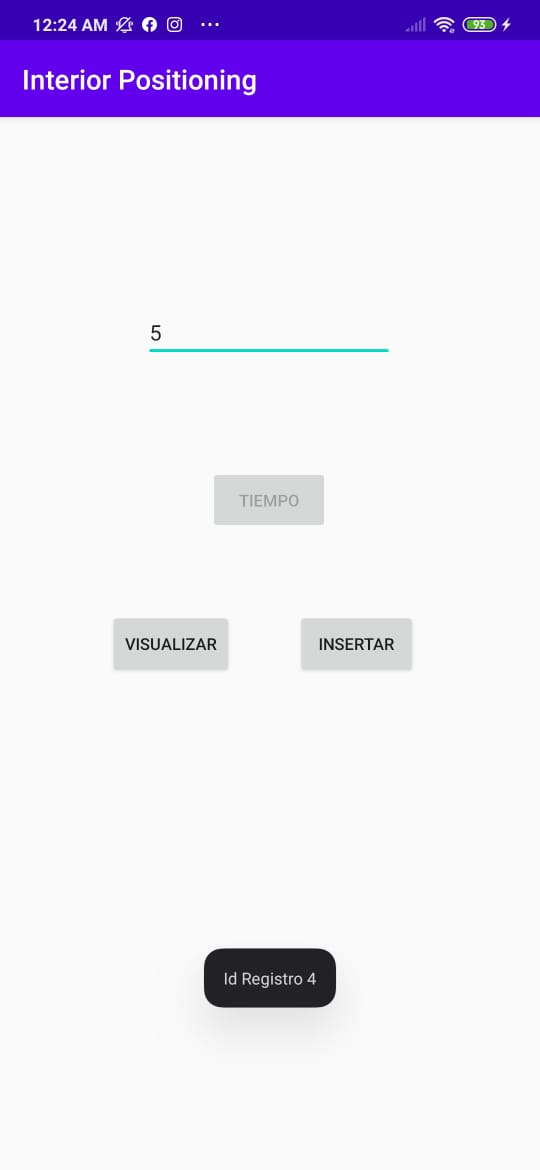
\includegraphics[scale=0.5]{bib/6.PNG}
    \label{fig:1}
\end{figure}
\begin{figure}[H]
    \centering
    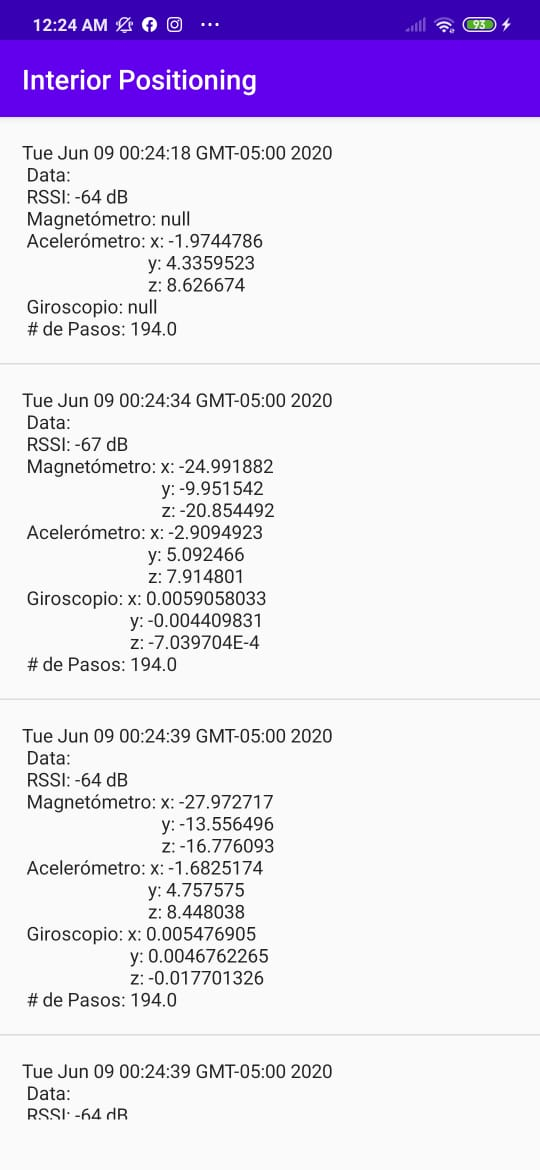
\includegraphics[scale=0.5]{bib/7.PNG}
    \label{fig:1}
\end{figure}
\begin{figure}[H]
    \centering
    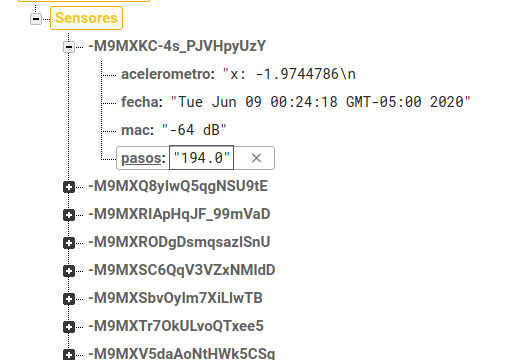
\includegraphics[scale=0.5]{bib/8.PNG}
    \label{fig:1}
\end{figure}

\begin{figure}[H]
    \centering
    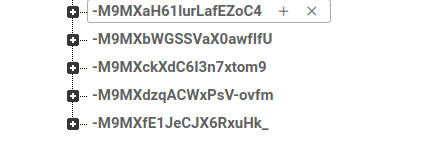
\includegraphics[scale=0.5]{bib/9.PNG}
    \label{fig:1}
\end{figure}
\begin{figure}[H]
    \centering
    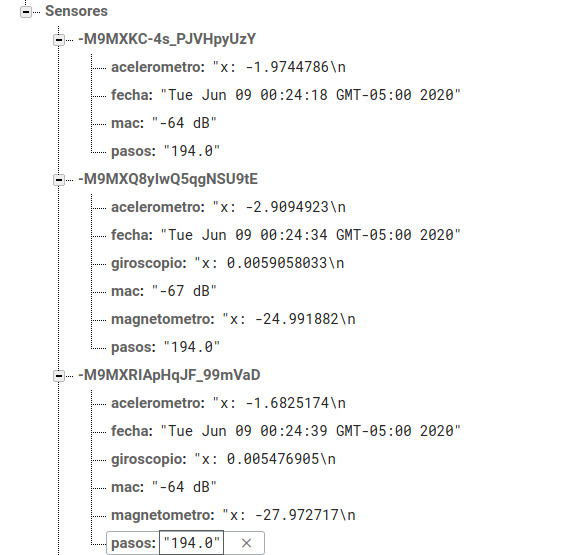
\includegraphics[scale=0.5]{bib/10.PNG}
    \label{fig:1}
\end{figure}


\textbf{Video de presentación:} https://youtu.be/bu88vWp8WJk


\nocite{*}
\bibliographystyle{IEEEtran}
\label{sec:biblio}
% Descomente y modiffique el archivo biblio.bib para agregar bibliografía
\bibliography{bib/biblio} 





%\pagestyle{empty}
\end{document}


